\section{Background information} % FIXME: improve name
\begin{frame}[t]{Definitions}{Some subtitle} % FIXME
	\begin{description}
		\item[Jayvee] A language aiming to allow everyone to describe ETL pipelines \footcite{jvalue:jayvee}.
		\item[ETL Pipeline] Extract the data
		\item[Columnar, column oriented] Values are saved column after column \footcite{Floratou2019}.
		      \begin{figure}
			      \begin{subfigure}{0.45\linewidth}
				      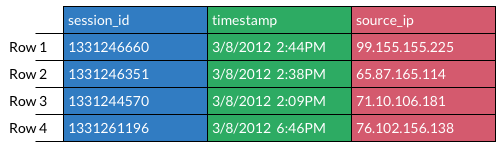
\includegraphics[width=0.9\linewidth]{assets/table-example.png}
				      \caption{An example table}
			      \end{subfigure}
			      \begin{subfigure}{0.22\linewidth}
				      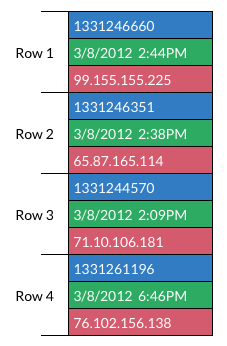
\includegraphics[height=0.3\FrameHeight]{assets/table-row.png}
				      \caption{The example table in a row-oriented format}
			      \end{subfigure}
			      \begin{subfigure}{0.22\linewidth}
				      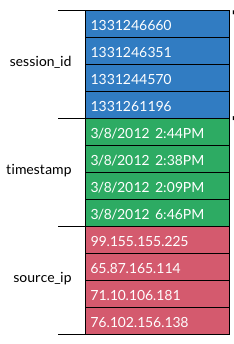
\includegraphics[height=0.3\FrameHeight]{assets/table-columnar.png}
				      \caption{The example table in a columnar format}
			      \end{subfigure}
			      \caption{Columnar and row-oriented memory layouts \footcite{arrow:overview}}
		      \end{figure}
	\end{description}
\end{frame}
